%
% Copyright (c) 2008 Betti Österholz
%
% Permission is granted to copy, distribute and/or modify this document
% under the terms of the GNU Free Documentation License, Version 1.2 or
% any later version published by the Free Software Foundation;
% with no Invariant Sections, no Front-Cover Texts, and no Back-Cover Texts.
%
% A copy of the license is included in the file ``fdl.tex'' .
%

%path for pictures
\graphicspath{{./material_enviroment/}}
\graphicspath{{./material_enviroment/}{../material_enviroment}}

\newpage
\part{Der genetische Algorithmus}\index{genetischer Algorithmus}\index{Algorithmus}
\label{secGeneticAlgorithmDesign}

In diesem Abschnitt werden allgemeine Entwurfsentscheidungen und erste Analysen für den genetischen Algorithmus aufgestellt.
Der realisierte genetische Algorithmus ist flexibel und erweiterbar gestaltet.

Der genetische Algorithmus ist natürlich auch ein evolutionärer Algorithmus. Die Bezeichnung ``genetisch'' bezieht sich auf die Fähigkeit des Algorithmus, Informationen von zwei oder mehr Individuen in einem neuen Individuum zu kodieren und darauf, dass er auf Informationen arbeitet, die ein (Multimedia-) Objekt kodieren und diese Objekte nicht direkt darstellen.

Der Algorithmus dient zur Erzeugung/Generierung von Fib-Objekten, welche ein Multimediaobjekt möglichst gut darstellen. Dem Algorithmus wird dafür ein bestimmtes Multimediaobjekt vorgegeben, für dass er Fib-Objekte/Individuen generiert, von denen gute selektiert werden. Die Generierung von Individuen kann auch Analysen des Multimediaobjekts beinhalten und die Nutzung oder Analyse von Informationen anderer Individuen. Welche Individuen gut sind, wird mithilfe von vorgegebenen Parametern entschieden (durch den Bewerter für Individuen).

\bigskip\noindent
Der Algorithmus besteht aus fünf separaten Teilen:
\begin{itemize}
 \item dem Kernalgorithmus
 \item dem Bewerter für Individuen
 \item dem Mortalitätsbewerter
 \item dem Bewerter für Operatoren
 \item der Menge der Operatoren
\end{itemize}

In der Abbildung \ref{figGeneticAlgorithmus} ist eine Ablaufskizze des genetischen Algorithmus dargestellt.

\begin{figure}[htbp]
\begin{center}
  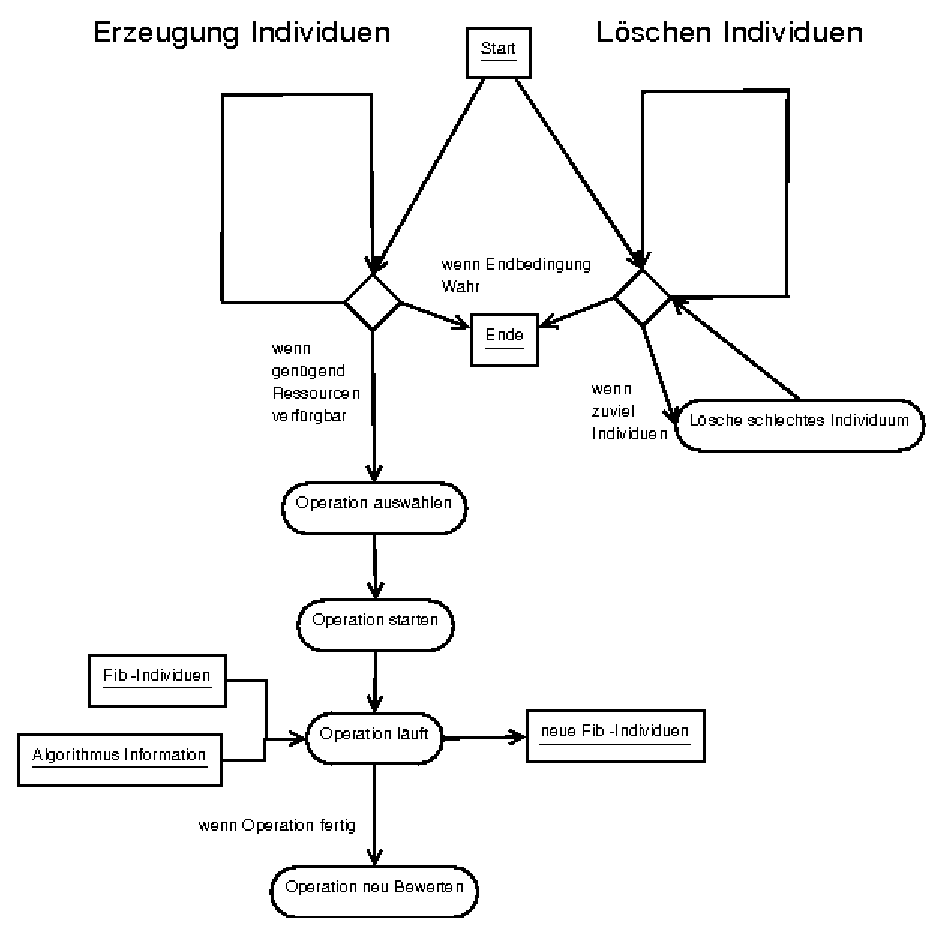
\includegraphics[scale=0.8]{algorithmus}
\end{center}
\caption{Ablaufskizze des genetischen Algorithmus}
\label{figGeneticAlgorithmus}
\end{figure}


Im Nachfolgenden werden die einzelnen Fib-Objekte als Individuen bezeichnet. Die Menge aller Individuen, die zu einem Zeitpunkt im Algorithmus vorhanden sind, wird kurz als Population bezeichnet.


\section{Kernalgorithmus}\index{Kernalgorithmus}

Der Kernalgorithmus nutzt die Bewerter und die Operatoren, um den genetischen Algorithmus zu realisieren. Er soll möglichst einfach gehalten und flexibel sein.

Die Bewerter für Individuen oder Operatoren sind (über Parameter) austauschbar.

\bigskip
Der Kernalgorithmus beinhaltet einmal die Hauptschleife des genetischen Algorithmus, in dem die Operatoren aufgerufen und Individuen erzeugt werden.

Als zweite Schleife existiert im Algorithmus die Selektionsschleife. Durch sie werden Individuen gelöscht.

\bigskip
Des Weiteren stellt der Kernalgorithmus Funktionen für die Operatoren bereit. Die Operatoren werden vom Kernalgorithmus über eine Methode aufgerufen, die für alle Operatoren gleich ist. Danach holen sich die Operatoren über Funktionen des Kernalgorithmus spezifische Werte aus dem Algorithmus, wie z. B. die Individuen, auf denen die Operationen arbeiten. Auf diese Weise sehen die Operatoren für den Kernalgorithmus immer jeweils gleich aus, und er benötigt keine Logik speziell für einen bestimmten Operator. Damit werden auch zukünftige Anpassungen der Operatoren vereinfacht, da nicht die Schnittstelle aller Operatoren angepasst werden muss, sondern nur die Funktionen, welche der Kernalgorithmus bereitstellt.

Die Aufrufmethode für die Operatoren soll flexibel sein, so dass auch Operatoren nebenläufig gestartet werden können und nicht auf die Beendigung jedes Operatoraufrufs gewartet werden muss. Die Operatoren sollten getrennt vom Kernalgorithmus laufen und diesen nur über die vorgegebene Schnittstelle beeinflussen können. Ein fehlerhafter Operator soll also nicht zu Fehlern im oder zur Beendigung des Gesamtsystems führen.


\section{Bewerten von Individuen}\index{Bewerter!Individuen}

Der konkrete Bewertungsalgorithmus sollte einfach auszutauschen sein, um verschiedenen Problemstellungen Rechnung tragen zu können. Der jeweilige Bewertungsalgorithmus wird zur Berechnung der Fitness eines Individuums benötigt.

Über Parameter für spezielle Bewerter können diese weiter angepasst werden (beispielsweise damit eingestellt werden kann, wie wichtig eine geringe Größe gegenüber eine schnellen Auswertung von Individuen ist).


\subsection{Die Fitness eines Individuums}

Die Fitness eines Individuums ist durch verschiedene Fitnessfaktoren gegeben.
Einer der wichtigsten ist, inwieweit das Individuum den gewünschten Originalmultimediadaten (z. B. dem Originalbild) ähnelt. Je mehr das Individuum (bzw. der Phänotyp dessen) den Originalmultimediadaten ähnelt, umso höher sollte die Fitness sein und umso geringer ist der Fehler, den das Individuum für die Darstellung der Originalmultimediadaten macht.

Dieser Fehler (und damit die Fitness des Individuums) kann z. B. über die Summe der (quadratischen) Abweichungen (nicht definierte Punkte liefern einen maximalen Fehler) in den Farben zu einem Punkt zwischen dem Originalbild und dem vom Individuum erzeugten Bild bestimmt werden oder über ein anderes selbstbestimmtes Abstandsmaß.

Wenn die Fitness für einzelne Teilobjekte des Individuums bestimmt wird, kann dies z. B. dadurch realisiert werden, dass in die Rechnung nur der Bereich einbezogen wird, der durch das Teilobjekt überdeckt wird, ein Rand um diesen Bereich noch mit einbezogen wird, oder auch nur das kleinste Quadrat benutzt wird, das dieses Objekt umschließt.

Ein anderer sinnvoller Fitnessfaktor ist die Größe (steigt mit der Anzahl der Elemente) der einzelnen Individuen, um größeren Individuen eine geringere Fitness zu geben als kleineren Individuen, mit dem gleichen Fehler auf den Originalmultimediadaten, und die kleineren Individuen so zu bevorzugen.

Ein weiterer Fitnessfaktor der einbezogen werden kann, ist eine Schätzung über die Zeit, die für das Individuum zur Berechnung des dargestellten Multimediaobjekts (Phänotyp) benötigt wird. Damit kann eventuell sogar die Ausführungsgeschwindigkeit des Algorithmus erhöht werden.


\subsection{Selektion durch Löschen von Individuen}\index{Selektion}

Um die Ressourcen (Arbeitspeicher, Rechenzeit) zu schonen, ist es notwendig, die Anzahl der Individuen (Fib-Objekte) im Bearbeitungsprozess (die noch am genetischen Algorithmus teilnehmen) zu beschränken. Deshalb müssen Individuen aus diesem nach Bedarf entfernt werden. Dabei sind Individuen mit einer niedrigen Fitness zu bevorzugen.

Deshalb gibt es für den Algorithmus einen \textbf{Mortalitätsbewerter}\index{Mortalitätsbewerter}. Dieser bestimmt, mit welcher Wahrscheinlichkeit ein Individuen gelöscht wird. Um Individuen zu löschen, gibt es im Algorithmus eine seperate Schleife, in der geprüft wird, ob die maximale Anzahl von Individuen überschritten ist. Wenn dies der Fall ist, werden so viele Individuen gelöscht, bis die maximale Anzahl von Individuen wieder eingehalten wird. Dabei haben Individuen mit einer hohen Bewertung durch den Mortalitätsbewerter auch eine hohe Wahrscheinlichkeit, gelöscht zu werden.

Der Mortalitätsbewerter orrientiert sich für seine Bewertung an der Fitness der Individuen. Er kann allerdings durch andere Mortalitätsbewerter ausgetauscht oder durch Parameter gesteuert werden. Es ist beispielsweise auch möglich, einige Individuen als unsterblich bzw. nicht löschbar zu deklarieren. Indem z. B. die $n$ ($n>0$) besten Individuen als unsterblich deklariert werden, kann vermieden werden, dass diese gelöscht werden und somit eines der besten Individuen verloren geht.

Der Mortalitätsbewerter kann weiterhin über die Operatorschnittstelle auf Statusinformationen des Algorithmus zugreifen, um z. B. die Anzahl der bisher erzeugten Individuen zu ermitteln.


\section{Bewerter für Operatoren}\index{Bewerter!Operatoren}

Um zu bestimmen, welcher Operator als nächstes ausgewählt wird, sind diese zu bewerten. Operatoren, die besser in einer Situation bewertet werden, haben eine höhere Wahrscheinlichkeit, in einer ähnlichen Situation ausgewählt bzw. ausgeführt zu werden.

\bigskip\noindent
Die Situation kann umfassen:
\begin{itemize}
 \item die wievielte Operation bzw. Interaktion ausgeführt wird.
 \item welcher Art das Originalmultimediaobjekt ist (über die Definitionen für die Umgebung in den root-Elementen dieses):
 \begin{itemize}
  \item es enthält Farben 
  \item es ist Schwarz/Weiß
  \item es enthält Ton
  \item es handelt sich um einen Film
  \item ...
 \end{itemize}
 \item die durchschnittliche (relative) Fitness der Individuen.
 \item die Fitness des besten/schlechtesten Individuums.
 \item die Standardabweichung der Fitnesswerte in der Population.
 \item die Anzahl der Individuen.
 \item Operationen, die bisher angewendet wurden.
 \item ...
\end{itemize}

Der spezielle Bewertungsalgorithmus kann ausgewählt werden. So können verschiedene Bewertungsalgorithmen leicht gegeneinander ausgetauscht und verglichen werden.

Zur Bewertung der Operatoren werden (von einzelnen Bewertern) eventuell Daten über ihre bisherigen Anwendungen permanent gehalten. Auf diese Weise kann der Algorithmus aus vorhergehenden Operatoraufrufen lernen.

Die Bewertung der Operatoren sollte möglichst Systemunabhängig erfolgen, also unabhängig vom Rechner, auf dem der Algorithmus gerade läuft.

\bigskip\noindent
Die Bewertungskriterien können sein:
\begin{itemize}
 \item Ausführungszeit der Operation
 \item erreichte Verschlechterungen oder Verbesserungen
 \item Zuverlässigkeit des Operators (Gibt er immer ein Ergebnis zurück? Stürzt er manchmal ab?)
 \item ...
\end{itemize}


\section{Die genetischen Operationen auf Fib}

Die Operatoren sind vom genetischen Algorithmus getrennt zu sehen. Es sollte möglich sein, beliebig viele Operatoren zum genetischen Algorithmus hinzuzufügen, ohne diesen anpassen zu müssen.

Jeder Operator hat eine eindeutige Kennung bzw. ID, über die ihm zugehörige Werte (z. B. seine bisherige Performance) zugeordnet werden können.

Wird ein Operator ausgeführt, ist dies eine Operation.

Diese Operationen sind dazu gedacht, Kodierungsalgorithmen zu implementieren. Operatoren sollten also nicht möglichst einfach sein, sondern können durchaus komplexe Algorithmen beinhalten.

Die Operatoren sollen auch möglichst zahlhaft sein, und der Algorithmus ist für die Auswahl guter Operatoren verantwortlich. Daher ist es auch erwünscht, mit sinvollen Teilen von Operatoren eigene Operatoren zu erstellen. Dabei sollten sowohl die Originaloperation als auch die Operation, die den Teil enthält, im Algorithmus verbleiben.

Für Spezialanwendungen kann ein genetischer Algorithmus verwendet werden, dessen Menge der Operatoren auf die nützlichsten für diese Anwendung eingeschränkt wurde.
Auch können für eine Anwendung nützliche Operatoren zu einem (nicht genetischen) Algorithmus kombinert werden, der diese in determinerter Weise verbindet.


\subsection{Vermehrung}

Bei der ``Vermehrung'' wird im Allgemeinen ein Individuum aus der Population genommen, bevorzugt Individuen mit hoher Fitness, dieses kopiert und durch Operationen verändert. Ist das entstehende Individuum ein ``neues'' Objekt (wenn es kein gleiches in der Population gibt), wird es zur Menge hinzugenommen. Es können auch bereits vorhandene Individuen übernommen werden.

Im Algorithmus wird die Vermehrung dadurch realisiert, dass eine Operation ausgeführt wird. Diese Operation holt sich dann über die Operationenschnittstelle vom Algorithmus alle benötigten Daten. Zu den benötigten Daten können ein oder mehrere Individuen gehören oder Daten über den bisherigen Verlauf des Algorithmus (z. B. die Nummer der bisherigen Interaktionen bzw. Operationen).


\section{Der soziale Aspekt des genetische Algorithmus}\index{Algorithmus!Sozialkomponente}

Die strikte Trennung der Operatoren vom Algorithmus und die Möglichkeit, Operationen leicht hinzufügen zu können, hat seinen Grund in eher sozialen Überlegungen.

Normale Kodierungsalgorithmen beschränken sich bei den Kodierungsmethoden auf eine oder nur wenige Ideen von einigen (in der Größenordnung von 1 bis 100) Menschen (dem Entwicklerteam). Da es aber viel mehr (in der Größenordnung von wahrscheinlich 100000) Menschen weltweit gibt, die sich im weiteren Sinne mit der effizenten Kodierung von Multimediaobjekten beschäftigen, bleiben dadurch zwangsläufig auch viele Ideen zur Kodierung unberücksichtigt. Selbst wenn ein Teil dieser Menschen daran Interesse hat, ihre Ideen einzubringen, ist dies nur sehr schwer bis unmöglich zu realisieren.

In den Fib-Algorithmus kann aber jeder neue Ideen in Form neuer Operatoren einbringen (ein Begriff dafür ist ``Crowdsourcing''). Dafür sind lediglich ausreichende Kenntnisse der Fib-Multi\-media\-beschrei\-bungs\-sprache und der Schnittstelle des Algorithmus für die Operatoren nötig. Um neue Ideen bzw. Operatoren zur effizenten Kodierung von Multimediaobjekten einzubringen, sollten keine Anpassungen am Allgorithmus oder anderen Operatoren nötig sein. Dadurch werden Seiteneffekte beschränkt und jede Implementierung einer Idee hat sich nur um die Idee bzw. deren Operator zu kümmern. Es sind also keine weiteren Kenntnisse des Algorithmus oder gar anderer Operatoren von Nöten. Auf diese Weise kann das System wachsen, ohne dass sich die Komplexität des (Kern-)Systems vergrößert und die Wartung und Erweiterung des Systems schwieriger wird.

Der Algorithmus und die Bildbeschreibungssprache sollten so angelegt sein, dass sich auch Laien ohne größeren Aufwand einarbeiten und neue Ideen bzw. Operatoren realisieren können. Insbesondere sollten Studenten und Studierende (z. B. Menschen mit Informatik als Hobby) der Informatik, sich innerhalb weniger Tage soweit einarbeiten können, dass sie einen eigenen Operator realisieren und einbinden können. (Wie nützlich oder effizient dieser ist, sei erst einmal dahingestellt.)

Die GNU-GPL-Lizenz, unter dem der Algorithmus steht, klärt die rechtliche Situation, unter der neue Operatoren stehen. Dadurch können neue Operatoren legal eingebunden werden, solange nicht andere Rechte verletzt werden (eine Verletzung wäre beispielsweise, dass in den Operatoren verwendete Algortihmen oder Codes unter inkompatiblen Lizenzen stehen). Neue Operatoren können auch der Allgemeinheit zur Verfügung gestellt werden.

Die Bewertung der Operatoren sollte motivieren, eigene Operatoren einzubinden. Dadurch kann jeder, der einen Operator hinzugefügt hat, realistisch einschätzen, wie gut sein Operator sich im Verhältnis zu anderen Operatoren in einer Situation macht. Der Wettbewerb unter Operatorenautoren sollte für neue bessere Operatoren förderlich sein.


All dies sollte dazu führen, dass nicht nur ein kleines Entwicklerteam zur Verbesserung der Kodierung von Fib-Objekten beiträgt, sondern dass ein viel größerer Kreis von Menschen sich mit diesen Thema beschäftigt. Dies sollte der Entwicklung und Verbreitung von Fib einen weiteren Schub geben.

In diesem Sinne ist der genetische Algorithmus für Fib ein transgenialer Algorithmus, der darauf angelegt ist, die Ideen von Menschen zur Kodierung von Multimediadaten aus deren Köpfen herauszuholen und in einem Topf zu transportieren/sammeln. Damit sollen diese Ideen/Algorithmen mehr leisten können, als sie es einzeln könnten. Der Algorithmus kann damit mehr Intelligenz in sich vereinen, als es ein Mensch (oder auch eine kleine Gruppe) hervorbringen kann.


\section{Warum sich genetische Algorithmen zur Multimediakodierung anbieten}

Es gibt im Allgemeinen keinen Algorithmus der Rastergrafiken direkt in speicherschonende Vektorbilder umwandeln kann, bei denen die Stärken der entsprechenden Vektorbeschreibungssprache wirklich genutzt werden. Für die Umwandlung von einem Multimediaformat in ein anderes ergibt sich oft eine ähnliche Problematik, insbesondere wenn das erste Multimediaformat die Eigenschaften von Punkten eines euklidischen (diskreten) Raumes direkt angibt (z. B. um Aufnahmen direkt abspeichern zu können) und das zweite Multimediaformat komplexe Objekte (z. B. Rechtecke oder/und Kreise) in Multimediaobjekten kodiert.

Da ein genetischer Algorithmus das Potential hat, alle möglichen Beschreibungen einer Multimediasprache zu generieren und unter diesen natürlich auch gute Beschreibungen sind, welche die Stärken der Multimediasprache in Bezug auf das Originalobjekt nutzen, hat ein genetischer Algorithmus natürlich auch das Potential, gute Beschreibungen zu generieren. Wenn im genetischen Algorithmus vorhandenes Wissen gut eingebaut wurde, kann er gute Beschreibungen wahrscheinlich auch schneller finden als eine reine Zufallssuche.

Noch ein weiterer Vorteil von genetischen Algorithmen ist die große Freiheit bei der Wahl der Problembeschreibung (Multimediasprache) und der möglichen Operatoren auf dieser. So kann völlig frei eine Multimediasprache nach eigenen Vorstellungen entworfen werden, die bestimmte Eigenschaften hat, z. B. Lesbarkeit, Einfachheit. Bei den Operatoren kann beliebig viel Wissen eingebaut werden. So ist es unter anderem auch möglich, schon bekannte gute Algorithmen zur Übersetzung von Rastergrafiken in Vektorbilder oder Teile von ihnen in Operatoren zu verwenden, so dass der genetische Algorithmus auf Rastergrafiken vom Ergebnis her mindestens so gut wird wie der verwendete Algorithmus, aber noch bessere Ergebnisse erzeugen kann.

Der große Nachteil von genetischen Algorithmen, dass sie sehr viel Zeit oder Rechenaufwand benötigen, wird dadurch abgeschwächt, dass dieser anfänglich hohe Aufwand ``billig'' sein kann und sich später auszahlt. Der genetische Algorithmus kann z. B. als Hintergrundprozess mit niedriger Priorität laufen, so dass er nur überflüssige Rechnerleistung verbraucht. Später kann durch das Ergebnis, das er geliefert hat, viel Übertragungsbandbreite eingespart werden.

Dies alles spricht für den Versuch, genetische Algorithmen zur Multimediakodierung zu verwenden.


\section{Komplexitätsabschätzung}
\label{abschaet}

Mit dem Ansatz aus Abschnitt \ref{secPowerOfFibOnPictures} auf Seite \pageref{secPowerOfFibOnPictures} kann eine beliebiges Rastergrafik in ein Fib-Objekt konvertiert werden, wobei der Kodierungsaufwand linear mit der Anzahl der Punkte und Eigenschaften wächst, da jeder Punkt mit seinen Eigenschaften einfach in ein Listenelement eingefügt werden kann und die Erzeugung der sonstigen Fib-Elemente (des root-Elements) konstante Zeit benötigt.

Dieser Ansatz ist auf beliebige Multimediadaten erweiterbar, die als Eigenschaften von Punkten eines endlichen, euklidischen, diskreten Raumes darstellbar sind. So kann immer ein Operator konstruiert werden, der ein Multimediaobjekt in linearer Zeit mit der Anzahl der Punkte und Eigenschaften in ein entsprechendes Fib-Objekt umwandelt. Dieses Fib-Objekt wächst auch von der Größe her nur linear mit der Anzahl der Punkte und Eigenschaften des Originalmultimediaobjekts.
Dieser Operator erzeugt allerdings keine effiziente Fib-Objektdarstellung, da er nicht die Möglichkeiten von Fib nutzt.

Wieviel Aufwand die Erzeugung besserer Fib-Objekte benötigt, kann nur schwer abgeschätzt werden, da sowohl die Operatoren als auch die Multimediaobjekte beliebig sein können. Es kann aber davon ausgegangen werden, dass für Multimediaobjekte mit einfacheren Strukturen der Aufwand auch geringer ist.


\section{Parallelen zur natürlichen Evolution}

Als Parallele seien hier die Bakterienstämme (z. B. E. coli) aufgeführt. Sie besitzen Gene, aufgrund derer bei ihnen genetische Evolution auftritt.

Bei diesen Bakterienstämmen (z. B. E. coli) kann es auch zu einem Gentransfer kommen, dabei wird ein Teil der Geninformationen (des Genmaterials oder dessen Kopien) von einer Bakterie zu einer anderen übertragen. Daneben gibt es natürlich auch Mutationsprozesse.

Ein Fib-Objekt kann als Information betrachtet werden, die ein Multimediaobjekt kodiert, so wie Bakteriengene eine Bakterie kodieren (Aufbau und Verhalten).

Die einzelnen Fib-Elemente sind dabei weniger als die Basen der Gene zu sehen, sondern vielmehr als die Funktionalität von Genen oder Genmengen. So wie bei den Bakterien durch Kombination der Gene bzw. der Dinge, die sie kodieren (z. B. Enzyme), erst komplexere Funktionalitäten definiert werden (z. B. Umsetzung von Zucker in Bewegungsenergie), entstehen bei Fib-Objekten erst durch Kombination der Elemente (Teil-)Multimediaobjekte (z. B. [Teil-]Bilder).

Fib-Teilobjekte können auch, wie beim Gentransfer bei den Bakterien, in andere Fib-Objekte übertragen werden und unterliegen einer Mutation, wobei auch bei den Bakterien schwer zu sagen ist, ob die Mutation der Gene wirklich völlig zufällig ist oder ob im Laufe der Jahrmillionen nicht Mechanismen entstanden sind, die zu einer ``intelligenteren'' Mutation führen, bzw. worin das zufällige Element besteht. Einzelne Fib-Objekte können dabei nicht nur als einzelne Bakterien angesehen werden, sondern auch als alle Bakterien mit identischen Geninformationen.

Das Originalmultimediaobjekt stellt die Nische dar, an welche sich die Bakterien anpassen sollen. Sie können dies auf viele unterschiedliche Arten tun, und die Anpassung muss auch nicht perfekt sein.

Allerdings werden beim genetischen Algorithmus für Fib-Objekte Operatoren angestrebt, die gezielte Verbesserungen vornehmen. Ein solcher explizit gerichteter Mechanismus ist bei Bakterien nicht zu erwarten.

Für weitere Informationen zur Genetik bei Bakterien sei auf ``Einführung in die Mikrobiologie''(\cite{genTrans}) verwiesen. Ein gutes Buch zur Evolution im allgemeinen ist ``Die Lösung von Darwins Dilemma'' \cite{LDD_2007} .
















